\def\Mu{\boldsymbol{\mu}}
\def\Lamb{\boldsymbol{\lambda}}

\lab{Interior Point 2: Quadratic Programs}{Interior Point 2: Quadratic Programs}
\objective{Interior point methods originated as an alternative to the Simplex method for solving linear optimization problems. However, they can also be adapted to treat convex optimization problems in general.
In this lab we implement a primal-dual Interior Point method for convex quadratic constrained optimization and explore applications in elastic membrane theory and finance.}

% Todo: change \geq in the constraints to the component-wise geq in the book.

\section*{Quadratic Optimization Problems}
%In this lab, we will explore an extension of Interior Point methods to a broader class of problems, namely quadratic constrained optimization problems.
A \emph{quadratic constrained optimization problem} differs from a linear constrained optimization problem only in that the objective function is quadratic rather than linear.
We can pose such a problem as follows:
\begin{align*}
\text{minimize }\qquad \frac{1}{2}&\x\trp Q\x + \c\trp \x\\
\text{subject to }\qquad &A\x \succeq \b,\\
&G\x = \mathbf{h}.
\end{align*}
% Unlike linear constrained optimization, the optimal point is not guaranteed to be one of the vertices of the feasible polytope (if the feasible region even is, indeed, a polytope).
% Thus, any attempt to extend the popular Simplex Algorithm to quadratic programs would require substantial adjustments, as that algorithm is crucially based on locating and searching through the vertices of the feasible region.
% Interior Point methods, however, generalize readily to the situation at hand.

We will restrict our attention to quadratic programs involving positive semidefinite quadratic terms (in general, indefinite quadratic objective functions admit many local minima, complicating matters considerably).
Such problems are called \emph{convex}, since the objective function is convex.
To simplify the exposition, we will also only allow inequality constraints (generalizing to include equality constraints is not difficult).
Thus, we have the problem
\begin{align*}
\text{minimize }\qquad \frac{1}{2}&\x\trp Q\x + \c\trp \x\\
\text{subject to }\qquad &A\x \succeq \b\\
\end{align*}
where $Q\in\mathbb{R}^{n\times n}$ is a positive semidefinite matrix, $A\in\mathbb{R}^{m\times n}$, $\x, \c \in \mathbb{R}^n$,
and $\b \in \mathbb{R}^m$.

%We begin by deriving the KKT conditions for this problem.
The Lagrangian function for this problem is:
\begin{align}
\mathcal{L}(\x,\Mu) = \frac{1}{2}\x\trp Q\x + \c\trp \x - \Mu\trp (A\x -\b),
\label{eq:lagrangian}
\end{align}
where $\Mu \in \mathbb{R}^m$ is the Lagrange multiplier.

\begin{comment} % Derivation overkill vvvvvvvvvvvvvvvvvvvvvvvvvvvvvvvvvvvvvvvvv
We next take the gradient of the Lagrangian with respect to $x$ and set it equal to zero:
\begin{align*}
0 &= \nabla_x \mathcal{L}(x,\lambda)\\
&= Qx + c - A\trp \lambda.
\end{align*}
We next write the complementary slackness condition:
\[
(Ax - b)_i\lambda_i = 0, \qquad i=1,2,\ldots,m.
\]
We finish by listing the inequality constraints as well as the nonnegativity constraint for $\lambda$:
\begin{align*}
Ax - b &\geq 0,\\
\lambda &\geq 0.
\end{align*}
\end{comment} % Derivation overkill ^^^^^^^^^^^^^^^^^^^^^^^^^^^^^^^^^^^^^^^^^^^

% What we have now is a mixture of equations and inequalities.
% We want to express these conditions as a system of equations, so
We also introduce a nonnegative slack vector $\y\in\mathbb{R}^m$ to change the inequality
$A\x - \b \succeq \0$ into the equality $A\x - \b - \y = \0$.

\begin{comment}
\begin{align}
A\x - \b - \y = \0 &&\Longrightarrow &&\y = A\x - \b
\label{eq:equality}
\end{align}
\end{comment}

Then the complete set of KKT conditions are:
% we make this substitution into the complementary slackness conditions.
% We obtain the following statement of the KKT conditions:
\begin{align*}
Q\x - A\trp \Mu + \c &= \0,\\
A\x - \b - \y &= \0,\\
y_i\mu_i &= 0, \qquad i=1,2,\ldots,m,\\
\y,\Mu &\succeq \0.
\end{align*}

\section*{Quadratic Interior Point Method}

The Interior Point method we describe here is an adaptation of the method we used with linear programming.
%The basic intuition is the same as before: we start at some point in the interior of the feasible region, and we make a series of steps so that we approach the solution to the KKT conditions iteratively.
% Since the solution to the KKT conditions can be seen as the root of a system of equations, our first thought might be to use Newton's Method for root-finding.
% This will not work on its own, however, because the KKT conditions also require inequality constraints, which will be violated if we blindly apply Newton's Method.
% Hence, we make adjustments to our choice of search direction and step size, so that we respect the constraints while moving closer to the solution of the KKT conditions.
Define $Y = \text{diag}(y_1,y_2,\ldots,y_m)$, $M = \text{diag}(\mu_1,\mu_2,\ldots,\mu_m)$, and let $\e\in\mathbb{R}^m$ be a vector of all ones.
Then the roots of the function
\begin{align*}
F(\x,\y,\Mu) =
\begin{bmatrix}
Q\x-A\trp \Mu + \c\\
A\x-\y-\b\\
YM\e
\end{bmatrix}
&= \0,\\
(\y,\Mu) &\succeq \0
\end{align*}
satisfy the KKT conditions.
The derivative matrix of this function is given by
\[
DF(\x,\y,\Mu) =
\begin{bmatrix}
Q & 0 & -A\trp \\
A & -I & 0\\
0 & M & Y
\end{bmatrix},
\]
and the duality measure $\nu$ for this problem is \[\nu = \frac{\y\trp \Mu}{m}.\]

\subsection*{Search Direction}

We calculate the search direction for this algorithm in the spirit of Newton's Method; this is the same way that we did in the linear programming case.
That is, we solve the system:
\begin{align}
DF(\x,\y,\Mu)
\begin{bmatrix}\triangle \x\\ \triangle \y\\ \triangle \Mu\end{bmatrix}
= - F(\x,\y,\Mu) +
\begin{bmatrix} \0 \\ \0 \\ \sigma\nu\e \end{bmatrix},
\label{eq:searchDirection}
\end{align}
where $\sigma\in [0,1)$ is the centering parameter.

\begin{problem}
Create a function \li{qInteriorPoint()}.
It should accept the arrays $Q, \c, A,$ and $\b$, a tuple of arrays \li{guess} giving initial estimates for $\x, \y,$ and $\Mu$ (this will be explained later), along with the keyword arguments \li{niter=20} and \li{tol=1e-16}.

In this function, calculate the search direction.
Create $F$ and $DF$ as described above, and calculate the search direction $(\triangle \x\trp , \triangle \y\trp , \triangle \Mu\trp )$ by solving Equation \ref{eq:searchDirection}.
Use $\sigma = \frac{1}{10}$ for the centering parameter.

(Hint: What are the dimensions of $F$ and $DF$?)
\end{problem}

\begin{comment} % Old method for search direction vvvvvvvvvvvvvvvvvvvvvvvvvvvvv
Our goal is to produce a sequence of points that approach the solution to this system of equations, all the while
respecting the nonnegativity constraints.% $\y,\Mu \geq \0$.
We achieve this goal using largely the same approach as in our linear programming Interior Point method.
We first apply Newton's method to $F$, obtaining a Newton search direction $(\triangle x, \triangle y, \triangle \lambda)$
that solves the system
\begin{equation}
\begin{bmatrix}
Q & 0 & -A\trp \\
A & -I & 0\\
0 & \Lambda & \mathcal{Y}
\end{bmatrix}
\begin{bmatrix}
\triangle x\\
\triangle y\\
\triangle \lambda
\end{bmatrix}
=
\begin{bmatrix}
-Qx + A\trp \lambda - c\\
-Ax + y + b\\
-\Lambda\mathcal{Y}e
\end{bmatrix}.
\label{eq:affine}
\end{equation}
We may not be able to step far in this direction without violating the nonnegativity constraints, so we calculate
an improved direction by perturbing the system of equations. This is done by making several small calculations.

First calculate the \emph{duality measure}
\[
\nu = \frac{1}{m}y\trp \lambda,
\]
which tells us about how close we are to the optimal point (values closer to zero indicate better proximity to the optimizer).

Next, we calculate a maximal allowed step length in the Newton direction:
\[
\hat{\alpha} = \max \{\alpha \in (0,1] \, | \, (y,\lambda) + \alpha(\triangle y, \triangle \lambda) \geq 0\}.
\]
You can check that this value is given by the minimum of the values
\begin{align*}
\min\left(1, \min_{i : \triangle y_i < 0} - \frac{y_i}{\triangle y_i}\right),\\
\min\left(1, \min_{i : \triangle \lambda_i < 0} -\frac{\lambda_i}{\triangle \lambda_i}\right).
\end{align*}

Continuing on, we compute the Newton duality measure given by
\[
\hat{\nu} = \frac{1}{m}(y + \hat{\alpha}\triangle y)\trp (\lambda + \hat{\alpha}\triangle \lambda),
\]
and then the centering parameter
\[
\sigma = \left(\frac{\hat{\nu}}{\nu}\right)^3.
\]

Finally, we obtain our search direction $(\triangle x', \triangle y', \triangle \lambda')$ by solving the perturbed
system
\begin{equation}
\begin{bmatrix}
Q & 0 & -A\trp \\
A & -I & 0\\
0 & \Lambda & \mathcal{Y}
\end{bmatrix}
\begin{bmatrix}
\triangle x'\\
\triangle y'\\
\triangle \lambda'
\end{bmatrix}
=
\begin{bmatrix}
-Qx + A\trp \lambda - c\\
-Ax + y + b\\
-\Lambda\mathcal{Y}e - \triangle \Lambda\triangle\mathcal{Y}e + \sigma\nu e
\end{bmatrix}.
\label{eq:perturbed}
\end{equation}
\end{comment} % Old method for search direction ^^^^^^^^^^^^^^^^^^^^^^^^^^^^^^^

\subsection*{Step Length}
Now that we have our search direction, we select a step length.
 We want to step nearly as far as possible
without violating the nonnegativity constraints.
However, we back off slightly from the maximum allowed step length
because an overly greedy step at one iteration may prevent a descent step at the next iteration.
Thus, we choose our step size
\[
\alpha = \max\{a \in (0,1] \, \mid \, \tau(\y,\Mu) +a(\triangle \y, \triangle \Mu) \succeq \0\},
\]
where $\tau \in (0,1)$ controls how much we back off from the maximal step length.
For now, choose $\tau = 0.95$.
In general, $\tau$ can be made to approach $1$ at each successive iteration.
This may speed up convergence in some cases.

% This is equivalent to the method of choosing a step direction used in the previous lab.
% In this case, however, we will use a single step length for all three of the parameters.
We wish to step nearly as far as possible without violating the problem’s constraints, as to remain in the interior of the feasible region.
First, we calculate the maximum allowable step lengths for $\mu$ and $\y$.

\begin{align*}
\beta_{\max} &= \min\{-\mu_i/\triangle \mu_i \mid \triangle \mu_i < 0 \}\\
\delta_{\max} &=\min\{-y_i/\triangle y_i \mid \triangle y_i < 0 \}
\end{align*}
% Since $\Mu,\y \geq \0$.
If all of the entries of $\triangle \mu$ are nonnegative, we let $\beta_{\max} = 1$.
Likewise, if all the entries of $\triangle \y$ are nonnegative, let $\delta_{\max}=1$.
Next, we back off from these maximum step lengths slightly:
\begin{align*}
\beta &= \min(1, \tau\beta_{\max})\\
\delta &= \min(1, \tau\delta_{\max})\\
\alpha &= \min(\beta, \delta)
\end{align*}
This $\alpha$ is our final step length.
Thus, the next point in the iteration is given by:
\[
(\x_{k+1}, \y_{k+1}, \Mu_{k+1}) = (\x_k, \y_k, \Mu_k) + \alpha(\triangle \x_k, \triangle \y_k, \triangle \Mu_k).
\]
This completes one iteration of the algorithm.

\begin{comment} % Put this back in?
\begin{info}
As with our Interior Point method for linear constrained optimization, the most expensive part of each iteration is solving the linear systems \ref{eq:affine} and \ref{eq:perturbed}.
Note, however, that these systems both have the same matrix on the left-hand side.
This allows us to factor the matrix just once per iteration, and use the factorization to solve both systems.
A more sophisticated implementation would likely split up these large systems of equations into a few smaller ones, and then use Cholesky-based factorizations.
To simplify matters, we suggest simply using as a first attempt an LU decomposition on the entire matrix.
\end{info}
\end{comment}

\subsection*{Initial Point}
The starting point $(\x_0, \y_0, \Mu_0)$ has an important effect on the convergence of the algorithm.
The code listed below will calculate an appropriate starting point:
\begin{lstlisting}
def startingPoint(G, c, A, b, guess):
    """
    Obtain an appropriate initial point for solving the QP
    .5 x\trp  Gx + x\trp  c s.t. Ax >= b.
    Parameters:
        G -- symmetric positive semidefinite matrix shape (n,n)
        c -- array of length n
        A -- constraint matrix shape (m,n)
        b -- array of length m
        guess -- a tuple of arrays (x, y, l) of lengths n, m, and m, resp.
    Returns:
        a tuple of arrays (x0, y0, l0) of lengths n, m, and m, resp.
    """
    m,n = A.shape
    x0, y0, l0 = guess

    # initialize linear system
    N = np.zeros((n+m+m, n+m+m))
    N[:n,:n] = G
    N[:n, n+m:] = -A.T
    N[n:n+m, :n] = A
    N[n:n+m, n:n+m] = -np.eye(m)
    N[n+m:, n:n+m] = np.diag(l0)
    N[n+m:, n+m:] = np.diag(y0)
    rhs = np.empty(n+m+m)
    rhs[:n] = -(G.dot(x0) - A.T.dot(l0)+c)
    rhs[n:n+m] = -(A.dot(x0) - y0 - b)
    rhs[n+m:] = -(y0*l0)

    sol = la.solve(N, rhs)
    dx = sol[:n]
    dy = sol[n:n+m]
    dl = sol[n+m:]

    y0 = np.maximum(1, np.abs(y0 + dy))
    l0 = np.maximum(1, np.abs(l0+dl))

    return x0, y0, l0
\end{lstlisting}
Notice that we still need to provide a tuple of arrays \li{guess} as an argument.
Do your best to provide a reasonable guess for the array $\x$, and we suggest setting $\y$ and $\Mu$ equal to arrays of ones.
We summarize the entire algorithm below.

\begin{algorithm}[H]
\begin{algorithmic}[1]
\Procedure{Interior Point Method for QP}{}
    \State \textrm{Choose initial point } $(\x_0, \y_0, \Mu_0)$.
    \While{$k <\ $\li{niters} and $\nu \ge\ $\li{tol}:}
        \State \textrm{Calculate the duality measure} $\nu$.
        \State \textrm{Solve \ref{eq:searchDirection} for the search direction} $(\triangle \x_k, \triangle \y_k, \triangle \Mu_k)$.
        \State \textrm{Calculate the step length} $\alpha$.
        \State $(\x_{k+1}, \y_{k+1}, \Mu_{k+1}) = (\x_k, \y_k, \Mu_k) + \alpha(\triangle \x_k, \triangle \y_k, \triangle \Mu_k).$
    \EndWhile
\EndProcedure
\end{algorithmic}
\label{alg:intPt2}
\end{algorithm}

\begin{problem}
Complete the implementation of \li{qInteriorPoint()}.
Return the optimal point $\x$ as well as the final objective function value.
% and \li{verbose}, a boolean value indicating whether or not to print the current objective function value ($ \frac{1}{2}x_k\trp Qx_k + c\trp x_k$) and duality measure ($\nu_k = \frac{1}{m}y_k\trp \lambda_k$) at each iteration.
% \end{problem}

Test your algorithm on the simple problem
\begin{align*}
\text{minimize }\qquad \frac{1}{2}x_1^2 + x_2^2 - &x_1x_2 - 2x_1 - 6x_2\\
\text{subject to }\qquad
-x_1-x_2 &\geq -2,\\
x_1-2x_2 &\geq -2,\\
-2x_1-x_2&\geq -3,\\
x_1, x_2 &\geq 0.
\end{align*}
In this case, we have for the objective function matrix $Q$ and vector $\c$,
\[
Q = \begin{bmatrix}
1 & -1\\
-1 & 2
\end{bmatrix},
\qquad
\c = \begin{bmatrix}
-2\\
-6
\end{bmatrix}.
\]
The constraint matrix $A$ and vector $\b$ are given by:
\[
A = \begin{bmatrix}
-1 & -1\\
1 & -2\\
-2 & -1\\
1 & 0\\
0 & 1
\end{bmatrix},
\qquad
\b = \begin{bmatrix}
-2\\
-2\\
-3\\
0\\
0
\end{bmatrix}.
\]
Use $\x = [.5, .5]$ as the initial guess.
The correct minimizer is $\left[\frac{2}{3}, \frac{4}{3}\right].$

(Hint: You may want to print out the duality measure $\nu$ to check the progress of the iteration).
\end{problem}
% We solve this problem with the following code:
% \begin{lstlisting}
% >>> # test out our algorithm
% >>> Q = np.array([[1,-1.],[-1,2]])
% >>> c = np.array([-2,-6.])
% >>> A = np.array([[-1, -1], [1, -2.], [-2, -1], [1, 0], [0,1]])
% >>> b = np.array([-2, -2, -3., 0, 0])
% >>> x = np.array([.5, .5])
% >>> y = np.ones(5)
% >>> mu = np.ones(5)
% >>> print qInteriorPoint(Q, c, A, b, (x,y,mu), niter=7, verbose=True)
% (array([ 0.66666668,  1.3333333 ]), -8.222222138159772)
% \end{lstlisting}
% Check that your function gives the same output.

\begin{info}
The Interior Point methods presented in this and the preceding labs are only special cases of the more general Interior Point algorithm.
The general version can be used to solve many convex optimization problems, provided that one can derive the corresponding KKT conditions and duality measure $\nu$.
\end{info}

\section*{Application: Optimal Elastic Membranes}
The properties of elastic membranes (stretchy materials like a thin rubber sheet) are of interest in certain fields of mathematics and various sciences.
A mathematical model for such materials can be used by biologists to study interfaces in cellular regions of an organism or by engineers to design tensile structures.
Often we can describe configurations of elastic membranes as a solution to an
optimization problem.
As a simple example, we will find the shape of a large circus tent by solving a quadratic constrained optimization problem using our Interior Point method.

Imagine a large circus tent held up by a few poles.
We can model the tent by a square two-dimensional grid, where each grid point has an associated number that gives the height of the tent at that point.
At each grid point containing a tent pole, the tent height is constrained to be at least as large as the height of the tent pole.
At all other grid points, the tent height is simply constrained to be greater than zero (ground height).
In Python, we can store a two-dimensional grid of values as a simple two-dimensional array.
We can then flatten this array to give a one-dimensional vector representation of the grid.
If we let $\x$ be a one-dimensional array giving the tent height at each grid point, and $L$ be the one-dimensional array giving the underlying tent pole structure (consisting mainly of zeros, except at the grid points that contain a tent pole), we have the linear constraint: \[\x \succeq L.\]

\begin{figure}
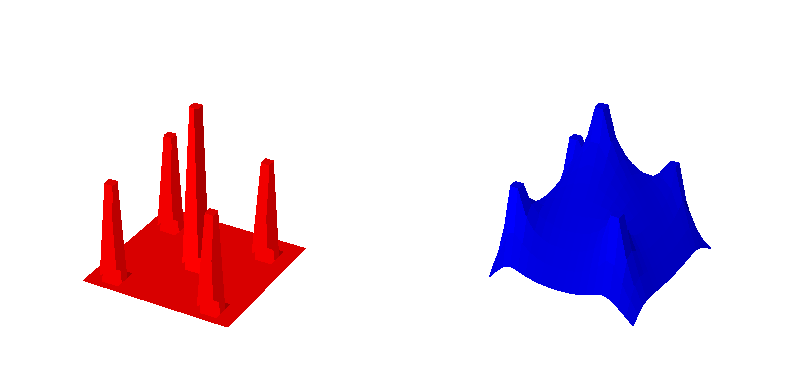
\includegraphics[width=\textwidth]{figures/tent.pdf}
\caption{Tent pole configuration (left) and optimal elastic tent (right).}
\label{fig:tent}
\end{figure}

The theory of elastic membranes claims that such materials tend to naturally minimize a quantity known as the \emph{Dirichlet energy}.
This quantity can be expressed as a quadratic function of the membrane.
Since we have modeled our tent with a discrete grid of values, this energy function has the form \[\frac{1}{2}\x\trp  H \x + \c\trp  \x,\] where $H$ is a particular positive semidefinite matrix closely related to Laplace's Equation, $\c$ is a vector whose entries are all equal to $-(n-1)^{-2}$, and $n$ is the side length of the grid.
Our circus tent is therefore given by the solution to the quadratic constrained optimization problem:
\begin{align*}
\text{minimize }\qquad &\frac{1}{2}\x\trp  H \x + \c\trp  \x\\
\text{subject to }\qquad &\x \succeq L.\\
\end{align*}
See Figure \ref{fig:tent} for an example of a tent pole configuration and the corresponding tent.

We provide the following function for producing the Dirichlet energy matrix $H$.
\begin{lstlisting}
from scipy.sparse import spdiags
def laplacian(n):
    """Construct the discrete Dirichlet energy matrix H for an n x n grid."""
    data = -1*np.ones((5, n**2))
    data[2,:] = 4
    data[1, n-1::n] = 0
    data[3, ::n] = 0
    diags = np.array([-n, -1, 0, 1, n])
    return spdiags(data, diags, n**2, n**2).toarray()
\end{lstlisting}
Now we initialize the tent pole configuration for a grid of side length $n$, as well as initial guesses for $\x$, $\y$, and $\Mu$.
\begin{lstlisting}
# Create the tent pole configuration.
>>> L = np.zeros((n,n))
>>> L[n//2-1:n//2+1,n//2-1:n//2+1] = .5
>>> m = [n//6-1, n//6, int(5*(n/6.))-1, int(5*(n/6.))]
>>> mask1, mask2 = np.meshgrid(m, m)
>>> L[mask1, mask2] = .3
>>> L = L.ravel()

# Set initial guesses.
>>> x = np.ones((n,n)).ravel()
>>> y = np.ones(n**2)
>>> mu = np.ones(n**2)
\end{lstlisting}
We leave it to you to initialize the vector $\c$, the constraint matrix $A$,
%(it's just the identity matrix of appropriate size)
and to initialize the matrix $H$ with the \li{laplacian()} function.
We can solve and plot the tent with the following code:
\begin{lstlisting}
>>> from matplotlib import pyplot as plt

# Calculate the solution.
>>> z = qInteriorPoint(H, c, A, L, (x,y,mu))[0].reshape((n,n))

# Plot the solution.
>>> domain = np.arange(n)
>>> X, Y = np.meshgrid(domain, domain)
>>> fig = plt.figure()
>>> ax1 = fig.add_subplot(111, projection='3d')
>>> ax1.plot_surface(X, Y, z,  rstride=1, cstride=1, color='r')
>>> plt.show()
\end{lstlisting}

\begin{problem}
Solve the circus tent problem with the tent pole configuration given above, for grid side length $n = 15$.
Plot your solution.
\end{problem}

\section*{Application: Markowitz Portfolio Optimization}
Suppose you have a certain amount of money saved up, with no intention of consuming it any time soon.
What will you do with this money?
If you hide it somewhere in your living quarters or on your person, it will lose value over time due to inflation, not to mention you run the risk of burglary or accidental loss.
A safer choice might be to put the money into a bank account.
That way, there is less risk of losing the money, plus you may even add to your savings through interest payments from the bank.
You could also consider purchasing bonds from the government or stocks from various companies, which come with their own sets of risks and returns.
Given all of these possibilities, how can you invest your money in such a way that maximizes the return (i.e. the wealth that you gain over the course of the investment) while still exercising caution and avoiding excessive risk?
Economist and Nobel laureate Harry Markowitz developed the mathematical underpinnings and answer to this question in his work on modern portfolio theory.

A \emph{portfolio} is a set of investments over a period of time.
Each investment is characterized by a financial asset (such as a stock or bond) together with the proportion of wealth allocated to the asset.
An asset is a random variable, and can be described as a sequence of values over time.
The variance or spread of these values is associated with the risk of the asset, and the percent change of the values over each time period is related to the return of the asset.
For our purposes, we will assume that each asset has a positive risk, i.e. there are no \emph{riskless} assets available.

Stated more precisely, our portfolio consists of $n$ risky assets together with an allocation vector
$\x = (x_1,\ldots,x_n)\trp $, where $x_i$ indicates the proportion of wealth we invest in asset $i$.
By definition, the vector $\x$ must satisfy \[\sum_{i=1}^n x_i = 1.\]
Suppose the $i$th asset has an expected rate of return $\mu_i$ and a standard deviation $\sigma_i$.
The total return on our portfolio, i.e. the expected percent change in our invested wealth over the investment period, is given by
\[\sum_{i=1}^n \mu_ix_i.\]
We define the risk of this portfolio in terms of the covariance matrix $Q$ of the $n$ assets: \[\sqrt{\x\trp  Q \x}.\]
The covariance matrix $Q$ is always positive semidefinite and captures the variance and correlations of the assets.

Given that we want our portfolio to have a prescribed return $R$, there are many possible allocation vectors $\x$ that make this possible.
It would be wise to choose the vector minimizing the risk.
We can state this as a quadratic program:
\begin{align*}
\text{minimize }\qquad &\frac{1}{2}\x\trp Q\x\\
\text{subject to }\qquad &\sum_{i=1}^n x_i = 1\\
&\sum_{i=1}^n \mu_ix_i = R.\\
\end{align*}
Note that we have slightly altered our objective function for convenience, as minimizing $\frac{1}{2}\x\trp Q\x$ is equivalent to minimizing $\sqrt{\x\trp Q\x}$.
The solution to this problem will give the portfolio with least risk having a return $R$.
Because the components of $\x$ are not constrained to be nonnegative, the solution may have some negative entries.
This indicates short selling those particular assets.
If we want to disallow short selling, we simply include nonnegativity constraints, stated in the following problem:
\begin{align*}
\text{minimize }\qquad &\frac{1}{2}\x\trp Q\x\\
\text{subject to }\qquad &\sum_{i=1}^n x_i = 1\\
&\sum_{i=1}^n \mu_ix_i = R\\
&\x \succeq \0.
\end{align*}

Each return value $R$ can be paired with its corresponding minimal risk $\sigma$.
If we plot these risk-return pairs on the risk-return plane, we obtain a hyperbola.
In general, the risk-return pair of any portfolio, optimal or not, will be found in the region bounded on the left by the hyperbola.
The positively-sloped portion of the hyperbola is known as the
\emph{efficient frontier}, since the points there correspond to optimal portfolios.
Portfolios with risk-return pairs that lie to the right of the efficient frontier are inefficient portfolios, since we could either increase the return while keeping the risk constant, or we could decrease the risk while keeping the return constant.
See Figure \ref{fig:frontier}.

\begin{figure}[H]
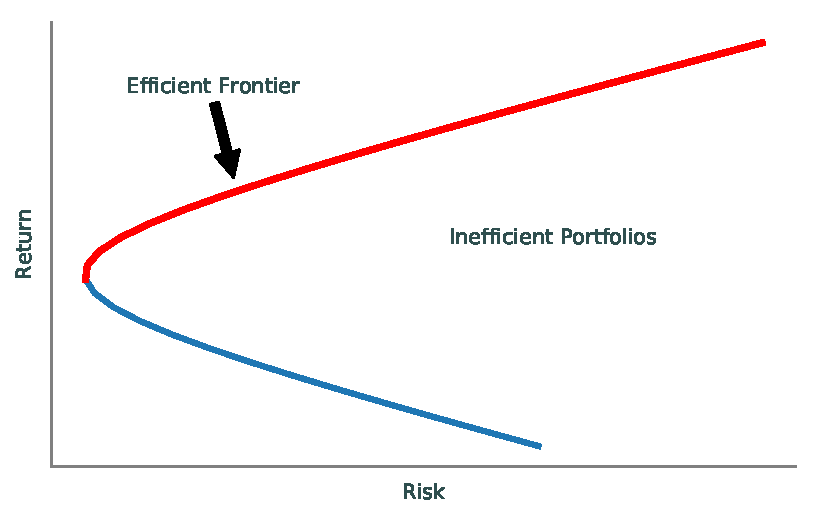
\includegraphics[width=0.75\textwidth]{figures/frontier.pdf}
\caption{Efficient frontier on the risk-return plane.}
\label{fig:frontier}
\end{figure}

One weakness of this model is that the risk and return of each asset is in general unknown.
After all, no one can predict the stock market with complete certainty.
There are various ways of estimating these values given past stock prices, and we take a very straightforward approach.
Suppose for each asset, we have $k$ previous return values of the asset. That is, for asset $i$, we have the data vector\[y^i = [y^i_1,\,\, \ldots, \,\,y^i_k]\trp .\]
We estimate the expected rate of return for asset $i$ by simply taking the average of $y_1,\ldots,y_k$, and we estimate the variance
of asset $i$ by taking the variance of the data.
We can estimate the covariance matrix for all assets by taking the covariance matrix of the vectors $y^1,\ldots,y^n$.
In this way, we obtain estimated values for each $\mu_i$ and $Q$.

\begin{problem}
The text file \li{portfolio.txt} contains historical stock data for several assets (U.S. bonds, gold, S\&P 500, etc).
In particular, the first column gives the years corresponding to the data, and the remaining eight columns give the historical returns
of eight assets over the course of these years.
Use this data to estimate the covariance matrix $Q$ as well as the expected rates of return $\mu_i$ for each asset.
Assuming that we want to guarantee an expected return of $R = 1.13$ for our portfolio, find the optimal portfolio both with and without short selling.

Since the problem contains both equality and inequality constraints, use the QP solver in CVXOPT rather than your \li{qInteriorPoint()} function.

Hint: Use \li{numpy.cov()} to compute Q.
\end{problem}
